\section{Auswertung}
\label{sec:Auswertung}

\subsection{Bestimmung der Abhängigkeit der Frequenzverschiebung zur Geschwindigkeit}  
In Tabelle \ref{tab:7mm} sind die gemessenen Werte für die Freuqenzverschiebungen der Winkel $\alpha_1=\qty{15}{\degree}$, $\alpha_2=\qty{30}{\degree}$ und $\alpha_3=\qty{45}{\degree}$ abhängig vpn der Pumpleistung  aufgeführt.
Diese Werte sind bei einem Rohrabschnitt, welcher einen Durchmesser von $d_1=\qty{7}{\milli\meter}$ besitzt, aufgenommen.

\begin{table}[H]
  \centering
  \caption{Aufgeführt sind die Freuqenzverschiebungen der verschiedenen Winkel, abhängig von der Pumpleistung, für einen Rohrdurchmesser von $\qty{7}{\milli\meter}$.}
  \label{tab:7mm}
  \sisetup{table-format=1.1, per-mode=reciprocal}
  \begin{tblr}{
      colspec = {S[table-format=1.0] S[table-format=4.0] S[table-format=4.0] S[table-format=5.0]},
      row{1} = {guard, mode=math},
      }
      \toprule
      P_{Pump} \mathbin{/} \unit{\liter\per\minute} & \increment \nu_{15} \mathbin{/} \unit{\hertz} & \increment \nu_{30} \mathbin{/} \unit{\hertz} & \increment \nu_{45} \mathbin{/} \unit{\hertz} \\
      \midrule
      3     &  220 &  476  &  922 \\
      4     &  317 &  708  & 1465 \\
      5     &  415 & 1007  & 2039 \\
      6     &  580 & 1379  & 2625 \\
      7     &  708 & 1660  & 3284 \\
      \bottomrule
  \end{tblr}
\end{table}

Für den Rohrabschnitt mit $d_2=\qty{16}{\milli\meter}$ sind die Werte in Tabelle \ref{tab:10mm} eingetragen.

\begin{table}[H]
  \centering
  \caption{Hier sind die Freuqenzverschiebungen abhängig von der Pumpleistung aufgelistet, bei einem Rohrdurchmesser von $\qty{16}{\milli\meter}$ und bei verschiedenen Winkeln.}
  \label{tab:10mm}
  \sisetup{table-format=1.1, per-mode=reciprocal}
  \begin{tblr}{
      colspec = {S[table-format=1.0] S[table-format=4.0] S[table-format=4.0] S[table-format=5.0]},
      row{1} = {guard, mode=math},
      }
      \toprule
      P_{Pump} \mathbin{/} \unit{\liter\per\minute} & \increment \nu_{15} \mathbin{/} \unit{\hertz} & \increment \nu_{30} \mathbin{/} \unit{\hertz} & \increment \nu_{45} \mathbin{/} \unit{\hertz} \\
      \midrule
      3   &        85  & 122 & 195  \\
      4   &       122  & 195 & 317  \\
      5   &       171  & 269 & 439  \\
      6   &       220  & 342 & 604  \\
      7   &       269  & 439 & 787  \\
      \bottomrule
  \end{tblr}
\end{table}

Dann wurde die Gleichung \ref{eqn:verschiebung2} zu
\begin{equation}
  \frac{\increment \nu}{\cos{\alpha}} = k \cdot v \, , k=\frac{2 v_0}{c}
  \label{eqn:verschiebung3}
\end{equation} 
umgeformt.
$\alpha$ wurde mit Formel \ref{eqn:winkel} berechnet.

Die Konstante $k$ wird mithilfe einer Ausgleichsgeraden bestimmt.
Dafür musste $v$ mithilfe von Gleichung \ref{eqn:geschwindigkeit} und 
\begin{equation*}
  A=\pi \cdot (\frac{d}{2})^2
\end{equation*}
\noindent ausgerechnet werden.

Der Rechte Teil von Gleichung \ref{eqn:verschiebung3} wird dann gegen $v$ aufgetragen und eine lineare Regression durchgeführt.
Dies wird für die verschiedenen Winkel und für die verschiedenen Winkel bei $d_2$ analog gemacht.
Abgebildet ist dies in \ref{fig:plot}.


\begin{figure}
  \centering
  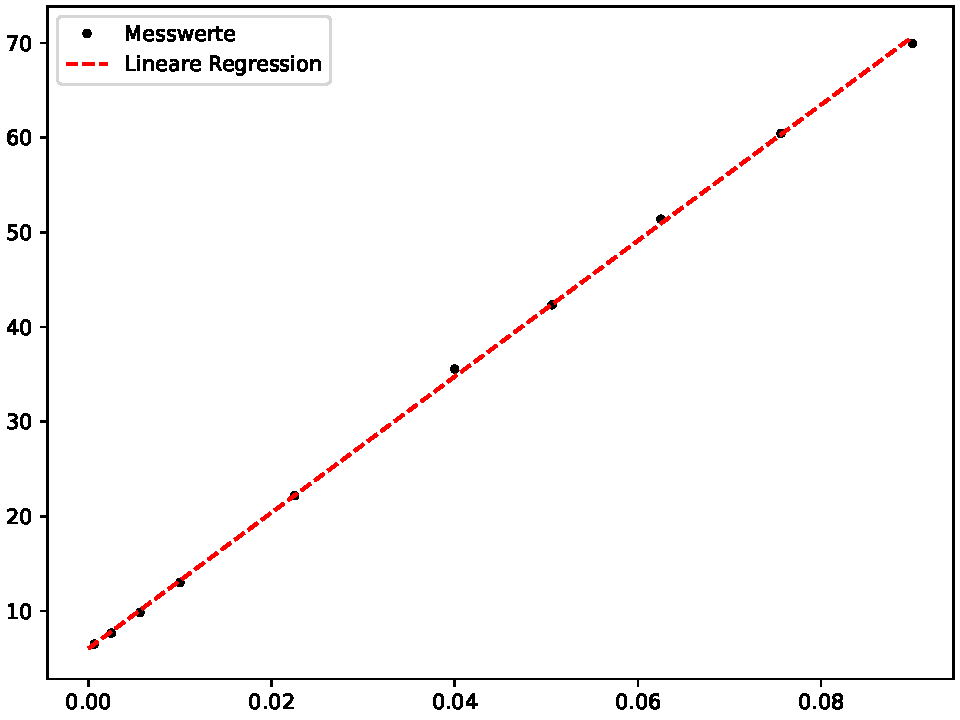
\includegraphics{plot.pdf}
  \caption{Abgebildet ist der Quotient von der Frequenzverschiebung und dem Cosinus von $\alpha$ in Abhängigkeit zur Flussgeschwindigkeit $v$.
  Zudem qurde jeweils eine Ausgleichsgerade hinzugefügt.}
  \label{fig:plot}
\end{figure}

\noindent Mithilfe einer Ausgleichsgeraden wird dann die Steigung bestimmt.
Damit folgt $k_e=\qty{1615.66(156.37)}{\hertz}$.


Ein theoretischer Wert von $k$ lässt sich mit 
\begin{equation*}
  k=\frac{2 v_0}{c}
\end{equation*}
\noindent berechnen. 
Dabei ergibt sich $k_t=\qty{1481.48}{\hertz}$.


\subsection{Bestimmung des Strömungsprofils}

Um das Strömungsprofil zu bestimmen, wird die Frequenzverschiebung abhängig von der Messzeit aufgenommen.
Die Werte sind in den Tabellen \ref{tab:Profil1} und \ref{tab:Profil2} aufgelistet.
Dabei befinden sich in Tabelle \ref{tab:Profil1} die Messwerte für einen Rohrdurchmesser von $d=\qty{10}{\milli\meter}$ und in \ref{tab:Profil2} 
die für $d=\qty{7}{\milli\meter}$, jeweils für Pumpleistungen von $3$ und $\qty{6}{\liter\per\minute}$.

\begin{table}[http]
  \centering
  \caption{Aufgelistet sind die Frequenzverschiebungen bei einem Rohrdurchmesser von $10mm$ abhängig von der Messzeit.}
  \label{tab:Profil1}
  \begin{minipage}[t]{0.4\textwidth}
    \begin{adjustwidth}{1.cm}{}
    \begin{tblr}[t]{
      colspec = {S[table-format=1.0] S[table-format=4.0] },
      row{1} = {guard, mode=math},
    }
    \toprule
      t \mathbin{/} \unit{\micro\second}  & \increment \nu_3 \mathbin{/} \unit{\hertz} \\
    \midrule
    13.5   &   0 \\
    14.0   & 171 \\
    14.5   & 183 \\
    15.0   & 208 \\
    15.5   & 220 \\
    16.0   & 195 \\
    16.5   & 183 \\
    17.0   & 159 \\
    17.5   & 134 \\
    18.0   & 122 \\
    18.5   &   0 \\
    \bottomrule
    \end{tblr}
    \end{adjustwidth}
  \end{minipage}
  \begin{minipage}[t]{0.4\textwidth}
    \begin{adjustwidth}{-0.5cm}{}
    \begin{tblr}[t]{
      colspec = {S[table-format=1.0] S[table-format=4.0] },
      row{1} = {guard, mode=math},
    }
    \toprule
      t \mathbin{/} \unit{\micro\second}  & \increment \nu_6 \mathbin{/} \unit{\hertz} \\
    \midrule
    12.5   &   0\\
    13.0   & 342\\
    13.5   & 427\\
    14.0   & 513\\
    14.5   & 574\\
    15.0   & 598\\
    15.5   & 610\\
    16.0   & 574\\
    16.5   & 513\\
    17.0   & 403\\
    17.5   & 330\\
    18.0   & 293\\
    18.5   & 281\\
    19.0   & 350\\
    19.5   & 391\\
    \bottomrule
    \end{tblr}
    \end{adjustwidth}
  \end{minipage}
\end{table}

\begin{table}[http]
  \centering
  \caption{Aufgeführt sind ist hier die Frequenzverschiebungen für $d=7cm$ abhängig von $t$.}
  \label{tab:Profil2}
  \begin{minipage}{0.4\textwidth}
    \begin{adjustwidth}{1cm}{}
    \begin{tblr}{
      colspec = {S[table-format=1.0] S[table-format=4.0] },
      row{1} = {guard, mode=math},
    }
    \toprule
      t \mathbin{/} \unit{\micro\second}  & \increment \nu_3 \mathbin{/} \unit{\hertz} \\
    \midrule
    13.0 &     0\\
    13.5 &   452\\
    14.0 &   537\\
    14.5 &   623\\
    15.0 &   696\\
    15.5 &   671\\
    16.0 &   586\\
    16.5 &   488\\
    17.0 &   415\\
    17.5 &   372\\
    18.0 &   391\\
    18.5 &   403\\
    19.0 &   409\\
    19.5 &   470\\
    \bottomrule
    \end{tblr}
    \end{adjustwidth}
  \end{minipage}
  \begin{minipage}{0.4\textwidth}
    \begin{adjustwidth}{-0.5cm}{}
    \begin{tblr}{
      colspec = {S[table-format=1.0] S[table-format=4.0] },
      row{1} = {guard, mode=math},
    }
    \toprule
      t \mathbin{/} \unit{\micro\second}  & \increment \nu_6 \mathbin{/} \unit{\hertz} \\
    \midrule
    13.0   &    0\\
    13.5   & 1050\\
    14.0   & 1270\\
    14.5   & 1453\\
    15.0   & 1611\\
    15.5   & 1636\\
    16.0   & 1447\\
    16.5   & 1221\\
    17.0   & 1062\\
    17.5   &  983\\
    18.0   & 1001\\
    18.5   & 1038\\
    19.0   & 1056\\
    19.5   & 1196\\
    \bottomrule
    \end{tblr}
    \end{adjustwidth}
  \end{minipage}
\end{table}


Da die Messtiefe in Acryl $\qty{4}{\micro\second}=\qty{10}{\milli\meter}$ entspricht, kann ab einer Zeit von $\qty{12.28}{\micro\second}$ die Umrechnung der Dopplerphantomflüssigkeit genutzt werden.
Diese entspricht $\qty{4}{\micro\second}=\qty{7}{\milli\meter}$.
Die $\qty{12.28}{\micro\second}$ werden dann von der gemessenen Zeit abgezogen, da sich erst nach dieser Zeit die Schallwellen an der Flüssigkeit befinden.
Die Geschwindigkeit wird mit Formel \ref{eqn:geschwindigkeit} berechnet.
Nun wird die Geschwindigkeit gegen die Messtiefe aufgetragen.
Dabei ergeben sich die Profile in \ref{fig:Profile}
\begin{figure}
  \centering
  \includegraphics[width=\textwidth]{profil.pdf}
  \caption{Hier ist die Geschwindigkeit der Flüssigkeit im Rohr zur Messtiefe aufgetragen.}
  \label{fig:Profile}
\end{figure}